\documentclass[10pt,a4paper]{article}
\usepackage[utf8]{inputenc}
\usepackage{amsmath}
\newcommand{\RomanNumeralCaps}[1]
    {\MakeUppercase{\romannumeral #1}}
\usepackage{amsfonts}
\usepackage{amssymb}
\usepackage{float}
\usepackage{verbatim}
\usepackage{listings}
\usepackage{hyperref}

\usepackage{color} %red, green, blue, yellow, cyan, magenta, black, white
\definecolor{mygreen}{RGB}{28,172,0} % color values Red, Green, Blue
\definecolor{mylilas}{RGB}{170,55,241}
\usepackage{amsmath}
\usepackage{graphicx}
\graphicspath{{C:/Users/adria/Pictures/FYS3150/}} 
\author{Adrian Martinsen Kleven, Simon Schrader}
\title{Project 2}

\lstset{
 	language =C++,   
    frame=tb, % draw a frame at the top and bottom of the code block
    tabsize=4, % tab space width
    showstringspaces=false, % don't mark spaces in strings
    numbers=left, % display line numbers on the left
    commentstyle=\color{green}, % comment color
    keywordstyle=\color{blue}, % keyword color
    stringstyle=\color{red} % string color
}

\begin{document}

\part*{-Project 2 - FYS3150/FYS4150-
}
{\large By Simon Schrader (4150), Adrian Kleven (3150) - autumn 2019
}
\tableofcontents

\listoffigures
\listoftables

 
\clearpage
 
\section{Abstract}

\section{Introduction}
\subsection{Purpose} 
The purpose of this report is to transform different problems arising in the physical sciences, such as simple quantum mechanical systems or a buckling beam, into problems that can be solved using methods from linear algebra and implement certain numerical algorithms, as well as test their efficiency.
Specifically, discretizing the radial Schroedinger equation bound by 3- dimensional harmonic oscillator potentialsinto a system of linear equations and restating the problem in terms of an eigenvalue problem.
\subsection{Approach}
Discretizing the Radial Schroedinger equation yields a set of linear equations that by the use of Dirichlet boundary conditions yield an eigenvalue problem of a tridiagonal Toeplitz- matrix. The relevance of this is that the eigenvalues of such a matrix have analytical solutions, which gives a benchmark by which the algorithms can be tested.\\The algorithms are implemented using C++, and we compare the time usage of our implementation with the time usage in the C++ library armadillo.
\section{Methods}

\subsection{Jacobi's eigenvalue algorithm}\label{jacobi algo}
This algorithm bases itself on the properties of similarity transformations. Assume a real and symmetric matrix $A$ with $n$ eigenvalues $\lambda_1,\lambda_2,...,\lambda_n$. Then there exists a real orthogonal matrix $S$ such that
\begin{equation}\label{eq:1}
S^TAS=\begin{bmatrix}
\lambda_1 & 0 & \cdots & 0 \\
0 & \lambda_2 & 0 & \vdots \\
\vdots & 0 & \ddots & 0 \\
0 & \cdots & 0 & \lambda_n \\
\end{bmatrix}.
\end{equation}
It can be shown then, that the $j'th$ column of the matrix $S$ is the eigenvector corresponding to the eigenvalue $\lambda_j$ for $j \in [1,2,...,n]$ see Ref. [3], chapter 8.\\\\A matrix $B$ is similar to $A$ if $B=S^{T}AS$, where $S$ is an orthogonal matrix. It can be shown that \hyperref[proof of same eigenvalues]{\emph{$B$ shares eigenvalues with $A$}}. Though the eigenvectors are not in general the same unless $S^T$ happens to be the identity matrix, but then this whole affair would be rather pointless.\\\\Using this property of the similarity transformation, successive applications of such a transform:
$$
S_N^TS_{N-1}^T...S_1^TAS_1...S_{N-1}S_N
$$
will retain the eigenvalues of the original matrix $A$. If in addition, the matrices $S$ and $S^T$ had the property that they gradually reduced the non- diagonal matrix elements to zero, then several iterations of this would yield a diagonal matrix with the eigenvalues of A along the diagonal ( equation \ref{eq:1} ).\\Such a matrix can be constructed by tailoring the orthogonal $(n\times n)$ rotation matrix
\begin{equation*}
\begin{bmatrix}
1 & 0 & \cdots & \cdots & \cdots & \cdots & 0 & 0\\ 
 0& 1 & 0 & \cdots &\cdots  &\cdots  &0  &0 \\ 
 \vdots& 0 & \ddots & \ddots & \vdots & \vdots & \vdots &\vdots \\ 
 \vdots& \cdots & \ddots & \cos\theta &0  & \cdots & 0 &\sin\theta \\ 
\vdots & \cdots & \cdots & \cdots & 1 & 0 & \cdots &0 \\ 
 \vdots& \cdots & \cdots & \cdots & \cdots & \ddots & \vdots & \vdots\\ 
0 & \cdots & \cdots &\cdots  & \cdots &\cdots  & 1 & 0\\ 
0 &\cdots  & 0 & -\sin\theta & 0 & \cdots & 0 & \cos\theta
\end{bmatrix}\hspace{2cm} ref.(2)
\end{equation*}
where the matrix elements that aren't zero are given by
$$
s_{kk}=s_{ll}=\cos\theta,s_{kl}=-s_{lk}=-\sin\theta,s_{ii}=-s_{ii}=1\hspace{1cm} i\neq k\hspace{1cm} i\neq l
$$
by changing the angle $\theta$ so as to make the non-diagonal matrix elements of $B$ equal to zero.\\After the transformation $B=S^TAS$ the matrix elements of $B$ are as follows:
$$
For \hspace{1cm} i\neq k,i \neq l
$$
$$
b_{ii} = a_{ii}
$$
$$
b_{ik} = a_{ik}\cos\theta - a_{il}\sin\theta
$$
$$
b_{il} = a_{il}\cos\theta + a_{ik}\sin\theta
$$
$$
b_{kk} = a_{kk}\cos^2\theta - 2a_{kl}\cos\theta \sin\theta + a_{ll}\sin^2\theta \hspace{1cm} ref. (2)
$$
$$
b_{ll} = a_{ll}\cos^2\theta + 2a_{kl}\cos\theta \sin\theta + a_{kk}\sin^2\theta \hspace{1cm}
$$
$$
b_{kl} = (a_{kk}-a_{ll})\cos\theta \sin\theta + a_{kl}(\cos^2\theta-\sin^2\theta) \hspace{1cm}
$$
$\theta$ is chosen such that the largest (by norm) off- diagonal matrix element $b_{mn}$ is set to zero. Then the other matrix elements of $B$ are calculated. This is then repeated for the new matrix $B$ with a new largest off- diagonal matrix element until the matrix $B$ resembles a diagonal matrix within a predetermined tolerance. As discussed above, the matrix $S$ which at this point equals the matrix product $S_1S_2...S_{N-1}S_N$, contains the eigenvectors corresponding to eigenvalues $\lambda_j$ in its j'th columns.
\subsection{The buckling beam problem}
A one- dimensional beam of length $L$ is secured at both ends ($x=0$ and $x=L$). A force $F$ is applied at the point $(L,0)$ in the $-x$ direction. The vertical displacement of the beam at a point $x$ is given by $u(x)$ where
$$
\gamma \frac{d^2 u(x)}{dx^2} = -F u(x).
$$
As the beam is fixed at both ends, the boundary conditions are $u(0)=u(L)=0$.$\gamma$ is related to the structural and material properties of the bar.\\it's helpful for computation to nondimensionalize the equation. An example of this can be seen \hyperref[nondim_2_el]{\emph{in the appendix}}.\\Firstly, the dimensionless variable $\rho =\frac{x}{L},\hspace{1mm} \rho \in [0,1]$ is introduced, making the new boundary conditions $u(0)=u(1)=0$. The eigenvalue is then set to\\$\lambda = \frac{FL^2}{\gamma}.$ The final expression is
\begin{equation*}
\frac{d^2u(\rho)}{d\rho^2}=-\lambda u(\rho).
\end{equation*} 
To discretize this expression, \hyperref[2nd derivative]{the equation for the second derivative} is applied.\\Given a number of mesh points $N$ the step length $h=\frac{1}{N}$ such that\\$\rho_i=ih, \hspace{1mm} i \in [1,2,...,N]$ and $u(\rho_i)=u_i$:
\begin{equation*}
-\frac{u_{i+1}-2u_i+u_{i-1}}{h^2}=\lambda u_i
\end{equation*}
This can be expressed in terms of the eigenvalue problem
\begin{equation*}
\begin{bmatrix}
d & a &0  &0  &\cdots  & 0\\ 
 a&  d& a & 0 & \cdots &0 \\ 
 0&  a&  d& \ddots  &\ddots  &\vdots \\ 
 0& 0 & a &  \ddots& a &0 \\ 
 \vdots&\vdots  &\ddots  &\ddots  &  d&a \\ 
 0& 0 & \cdots & 0 & a &d& 
\end{bmatrix}
  \begin{bmatrix} u_{1} \\
                                                              u_{2} \\
                                                              \vdots\\ \vdots\\ \vdots\\
                                                              u_{N-1}
             \end{bmatrix}=\lambda \begin{bmatrix} u_{1} \\
                                                              u_{2} \\
                                                              \vdots\\ \vdots\\ \vdots\\
                                                              u_{N-1}
             \end{bmatrix}.  
\end{equation*}
with $a = -\frac{1}{h^2}$ and $d=\frac{2}{h^2}$.\\It has analytical eigenvalues
\begin{equation*}
\lambda_j = d+2a\cos{(\frac{j\pi}{N+1})} \hspace{0.1cm} j=1,2,\dots N.
\end{equation*}
This will prove useful in testing the accuracy of the numerical algorithms later on.
\subsection{One electron in a 3- dimensional harmonic oscillator potential}
Assuming a centrally symmetric harmonic oscillator potential $V(r) = (1/2)m\omega^2r^2$ and a single electron with orbital angular moment equal to zero, the radial Schroedinger equation reads
\begin{equation*}
-\frac{\hbar^2}{2 m} \frac{1}{r^2} \frac{d}{dr} r^2\frac{d}{dr}R(r)+ V(r) R(r) = E R(r). \hspace{1cm} ref.(4)
\end{equation*}
From here on the equation is scaled in order to express the results in terms of dimensionless variables.\\
substituting $R(r) = (1/r) u(r)$. This simplifies the expression considerably to

\begin{equation*}
  -\frac{\hbar^2}{2 m} \frac{d^2}{dr^2}u(r)+ V(r) u(r) = E u(r).
\end{equation*}
Imposing Dirichlet boundary conditions, due to the nature of the normalizable wave functions that represent physical systems $u(0)=u(\infty)=0$. Dividing $r$ by the constant $\alpha$ where $[\alpha] = length$ to introduce the dimensionless variable $\rho =\frac{r}{\alpha}$, $V(\rho)$ becomes $\frac{1}{2}k\alpha^2 \rho^2$. The equation becomes

\begin{equation*}
  -\frac{\hbar^2}{2 m \alpha^2} \frac{d^2}{d\rho^2} u(\rho) 
       + \frac{k}{2} \alpha^2\rho^2u(\rho)  = E u(\rho) .
\end{equation*}
To get a factor of 1 in front the second derivative term, both sides of the equation are multiplied by $2m\alpha^2/\hbar^2$

\begin{equation*}
  -\frac{d^2}{d\rho^2} u(\rho) 
       + \frac{mk}{\hbar^2} \alpha^4\rho^2u(\rho)  = \frac{2m\alpha^2}{\hbar^2}E u(\rho) .
\end{equation*}
Then the value of $\alpha$ is fixed so that the factor in front of the second term on the LHS is 1

\begin{equation*}
\alpha = \left(\frac{\hbar^2}{mk}\right)^{1/4}.
\end{equation*}
Defining

\begin{equation*}
\lambda = \frac{2m\alpha^2}{\hbar^2}E,
\end{equation*}
Schroedinger's equation is then written as

\begin{equation*}
  -\frac{d^2}{d\rho^2} u(\rho) + \rho^2u(\rho)  = \lambda u(\rho) .
\end{equation*}
In order to discretize this, the expression for the second derivative

\begin{equation}
\label{2nd derivative}
  \frac{u(\rho+\epsilon) -2u(\rho) +u(\rho-\epsilon)}{\epsilon^2}
\end{equation}
is used.\\As infinity cannot be represented in a computer, a maximal value $\rho_{max}$ is used, at which the wave function approaches zero within a predetermined tolerance. Then, choosing a number of mesh points N from which the step length $h=\frac{\rho_N-\rho_0 }{N+1}$ is decided, $\rho$ can be discretized as $\rho_i= \rho_0 + ih$ where $i=1,2,\dots , N$ and $u(\rho_i)=u_i$. The following expression is then arrived at for the Schroedinger equation for a given $\rho_i$:

\begin{equation*}
-\frac{u_{i+1} -2u_i +u_{i-1}}{h^2}+\rho_i^2u_i= \lambda u_i
\end{equation*}
From here the matrix elements are defined from the coefficients of $u_{i+1}$, $u_{i}$, and $u_{i-1}$ .$u_0 = u(0)= 0$ and $u_N = u(\rho_{max}) \approx 0$ and so are exempt from the matrix, giving a $N-1 \times N-1$ matrix and corresponding eigenvalue problem:
$$
d_i=\frac{2}{h^2}+\rho_i^2,\hspace{1cm}  a=-\frac{1}{h^2}
$$
\begin{equation}
\label{discrete matrix}
\begin{bmatrix}
d_1 & a &0  &0  &\cdots  & 0\\ 
 a&  d_2& a & 0 & \cdots &0 \\ 
 0&  a&  d_3& \ddots  &\ddots  &\vdots \\ 
 0& 0 & a &  \ddots& a &0 \\ 
 \vdots&\vdots  &\ddots  &\ddots  &  d_{N-2}&a \\ 
 0& 0 & \cdots & 0 & a &d_{N-1}& 
\end{bmatrix}
  \begin{bmatrix} u_{1} \\
                                                              u_{2} \\
                                                              \vdots\\ \vdots\\ \vdots\\
                                                              u_{N-1}
             \end{bmatrix}=\lambda \begin{bmatrix} u_{1} \\
                                                              u_{2} \\
                                                              \vdots\\ \vdots\\ \vdots\\
                                                              u_{N-1}
             \end{bmatrix}.  
\end{equation}
From here, a number of algorithms can be used in fishing out the eigenvalues and corresponding eigenvectors. \hyperref[jacobi algo]{\emph{The Jacobi eigenvalue algorithm}} can be applied to any real, symmetric matrix, and so it will be applied here.
\subsection{Two electrons in a 3- dimensional harmonic oscillator potential}
For the case of two non- interacting electrons in a 3- dimensional harmonic oscillator potential, the Schroedinger equation can be written as 
\begin{equation*}
\left(-\frac{\hbar^2}{2 m} \frac{d^2}{dr_1^2}+ \frac{1}{2}k r_1^2\right)u(r_1,r_2)+\left( -\frac{\hbar^2}{2 m} \frac{d^2}{dr_2^2}+ \frac{1}{2}k r_2^2\right)u(r_1,r_2)  = E_{total} u(r_1,r_2).
\end{equation*}
When adding Coloumb interactions between the electrons, it's useful to introduce a set of new coordinates. $\vec{r}=\vec{r_1}-\vec{r_2}$ to capture the Coloumb interaction $V_C \propto ||\vec{r}||^{-1}$ and $R = \frac{\vec{r_1}+\vec{r_2}}{2}$, the average position of the two electrons in order to capture the energy associated with their position in the harmonic oscillator potential. The radial Schroedinger equation becomes (ref. (5))
\begin{equation*}
\left(  -\frac{\hbar^2}{m} \frac{d^2}{dr^2} -\frac{\hbar^2}{4 m} \frac{d^2}{dR^2}+ \frac{1}{4} k r^2+  kR^2\right)u(r,R)  = E_{total} u(r,R).
\end{equation*}
Where $E_{total} = E_r+E_R$ and $E_r$ is the energy associated with the electrons relative position and $E_R$ is the energy associated with their average position in the harmonic oscillator potential.\\The wave function $u(r,R)$ is separable by the ansatz into $\psi(r)\phi(R)$ and from here, only the r- dependent Schroedinger equation will be covered.\\\\The Coloumb repulsion is given by
\begin{equation*}
V(r)=\frac{\beta e^2}{r},
\end{equation*}
with the proportionality constants $\beta$ and $e$ given by $\beta e^2 = 1.44 eVnm$.\\Adding this to the potential energy of the Hamiltonian $\hat{H}_r$ gives
\begin{equation*}
\hat{H}_r= -\frac{\hbar^2}{m} \frac{d^2}{dr^2}+ \frac{1}{4}k r^2+\frac{\beta e^2}{r}
\end{equation*}
which in turn gives the radial time- independent Schroedinger equation
\begin{equation*}
\hat{H}_r \psi(r)=E_r\psi(r).
\end{equation*}
As was done for the case of the single electron, this equation will be nondimensionalized to aid in computation(\hyperref[nondim_2_el]{\emph{see Appendix}}).
Schroedinger's equation becomes
\begin{equation*}
  -\frac{d^2}{d\rho^2} \psi(\rho) + \omega_r^2\rho^2\psi(\rho) +\frac{1}{\rho}\psi(\rho) = \lambda \psi(\rho).
\end{equation*}
Using the \hyperref[2nd derivative]{\emph{equation for the second derivative}}, this equation can be discretized by the same method as for the single- electron case:
\begin{equation*}
-\frac{\psi_{i+1} -2\psi_i +\psi_{i-1}}{h^2}+\left( \omega_r^2 \rho_i^2+\frac{1}{\rho_i}\right)\psi_i= \lambda \psi_i
\end{equation*}
which makes for \hyperref[discrete matrix]{\emph{the same matrix as before}}, but now with
$$
d_i=\frac{2}{h^2}+\omega_r^2\rho_i^2 +\frac{1}{\rho_i}
$$

\subsection{ Implementation}
\subsubsection{Implementation of the Jacobi algorithm}
The implementation of the Jacobi algorithm is straightforward. Our implementation of the function takes the matrix takes four arguments: The (square) matrix A that needs to be diagonalized, the (square) matrix $R$ where the eigenfunctions are to be stored, the matrix dimension $n$, and a tolerance. Because the sum of the off-diagonal matrix elements get smaller for each orthogonal transformation, we decided to be done diagonalizing the matrix as soon as the maximum off-diagonal element is smaller than the tolerance. We set up $R$ to be the identity matrix.\\
Roughly speaking, the algorithm is implemented like this:\\
\begin{itemize}
\item[1.] Find the largest (absolute) non-diagonal element in A.
\item[2.] Set up the rotation matrix  $S$ to null out the largest non-zero element.
\item[3.] Set A  $\leftarrow$ $SAS^T$.
\item[4.] Set R $\leftarrow$ $S^TR$.
\item[5.] Go back to 1. until the largest (absolute) non-diagonal element in A is smaller than the tolerance.
\end{itemize}
\subsubsection{Implementation to solve the buckling beam problem}
For a given value n, We find the values for h, d and a using the formulas stated above. We are then able to state the matrix A, and apply the Jacobi algorithm to it. We start measuring the time right before calling our function to solve the jacobi algorithm, and we are done measuring the time right after. \\
We also ran the same set up using armadillo, where we did not call the Jacobi algorithm, but armadillo's $eig\_sym$-function.
\subsubsection{Appropriate values for $\rho$ and $n$ in the harmonic potential well}
The main difficulty was to find proper values for $n$ and $\rho_{max}$. Large values for $n$ decrease the computational error, as the step $h$ gets smaller, and we find more eigenvalues and eigenfunctions, but n increases computational time. A large $\rho_{max}$ decreases the error due to too early termination of the wave function, but also increases $h$, thus increasing the error for the formula of the second derivative, which is an approximation. We opted to choose values such that the error in the first  three eigenvalues for the electron in a 3- dimensional harmonic oscillator potential would be correct in the first 4 digits.
\subsubsection{One electron in a 3- dimensional harmonic oscillator potential}
The potential was set up as defined earlier and is a function of the distance $\rho$ and $\omega$ (which is 1 in one-electron case, but the same program was used for the two-electron-potential when the electron-electron term is ignored). \\
We chose n=400 and  $\rho_{max}=6$ to be sufficent in this case. The matrix $A$ is almost the same as for the buckling beam problem, but the potential was added to the diagonal elements as a function of $\rho$.
\subsubsection{Two electrons in a 3- dimensional harmonic oscillator potential}
The potential was set up to be the same as for the one-electron case, but the constant  $\omega^2$ was added to the quadratic term, and the term $1/r$ was added. We run the program for  $\omega$ $\in$ $[5,1,0.5,0.01]$. 
For $\omega$=5, we chose se n=400 and  $\rho_{max}=4$ to be sufficent. For $\omega=1$, wese considered n=400 and  $\rho_{max}=6$ to be sufficient.For $\omega=0.5$, $n=500$ and  $\rho_{max}=8$ gave good results. However, for ,$\omega=0.01$, we ended up using n=800 and   $\rho_{max}=40$. This is not ideal, but we ended up using these values, considering how larger values of  $\rho_{max}$ would decrease the accuracy due to an increased value of h, while increasing n would make the computational time skyrocket. 

\subsection{Unit testing}
We verified the correct implementation of the algorithm by checking three properties of a symmetric, fairly random $5\times 5$ matrix. We checked that our program to find the largest off-diagonal element worked correctly, we checked that we got the correct eigenvalues, and we checked that the eigenvectors were orthogonal, as orthogonal projections conserve the orthogonality of the eigenvectors (see appendix). 
\section{Results}
\subsection{Time usage}
We compared the time use of our implementation of the Jacobi algorithm to the eigen decomposition of a symmetric matrix as implemented in armadillo used to solve the harmonic oscillator, using the command eig\_sym. The time expenditure for different matrices of size $n\times n$ is shown in table 1:
\begin{table}[H]
\caption[Comparison of time use for algorithms]{Time usage in seconds for matrices of size $n\times n$ using the Jacobi algorithm vs. using armadillo's eig\_sym, averaged over 5 runs}
\begin{tabular}{lll}
$n$ &  armadillo & Jacobi algorithm \\
 10 & 0.0020 & 0.00025 \\
 100 & 0.056 & 0.45\\
 400 & 0.32 & 120
\end{tabular}
\end{table}
armadillo's implementation for solving symmetric positive-definite matrices is clearly much faster than the Jacobi algorithm. The time used to diagonalize a matrix  using the Jacobi algorithm for matrices of size $1000\times 1000$ or larger, is thus barely feasible on a personal computer, and implementing faster algorithms for the same general problem, or specializing the algorithm to a tridiagonal matrix, might be necessary. 
\subsection{Amount of orthogonal transformations}
The amount of necessary orthogonal transformations to diagonalize a matrix is assumed to be $3n^2-5n^2$ (see (2)) for the Jacobi algorithm for a matrix of size $n\times n$. Having a threshold of $10^{-8}$ for the largest element, we found that it takes roughly 15.000 orthogonal transformations for a matrix of size n=100, 60.000 for a matrix of size n=200, and 240.000 for a matrix of size n=400. These numbers increased only slightly when we changed the threshold to $10^{-12}$. This is clearly much less than expected, and we assume that the cause is the fact that we deal with a tridiagonal matrix, where most entries already are zeroed out. 
\subsection{Buckling beam}
We found that all eigenvalues were identical to the analytical solution with a relative error of less than $10^{-7}$. We did not do further research on that particular problem that already is well researched.
\subsection{one electron in three-dimensional harmonic oscillator well}
For the one-electron case, the eigenvalues for the ground state, the first excited state and the second excited state were found to be $\lambda_0=2.99993$ ,$ \lambda_1=6.99965$,$\lambda_2=10.9991$. Converted back to the original units, we thus get $E_0=1.49997\hbar\omega$, $E_1=3.49983\hbar\omega$, $E_2=5.49955\hbar\omega$. This data fits with the analytical solution to 3 decimals and indicates that our system was sat up correctly. The accuracy of these results could presumably be increased by increasing the cancellation condition in the algorithm, by increasing the matrix size n (thus decreasing h), and by increasing $\rho_{max}$. An interesting observation one can make here is that the eigenvalues get gradually less correct for the more excited states. The 9th excited state has an analytical eigenvalue $E_9=19.5\hbar\omega$, but our numerical approximation yields  $E_9=20.276\hbar\omega$. This is clearly incorrect and is caused by the boundary conditions, as infinity cannot be implemented. As one can see in figure 1, the squared eigenfunctions of the higher excited states get stretched out to larger values of $\rho$. Thus, the applied boundary conditions make the higher excited states go to zero where they are not supposed to be zero.
\begin{figure}[H]
	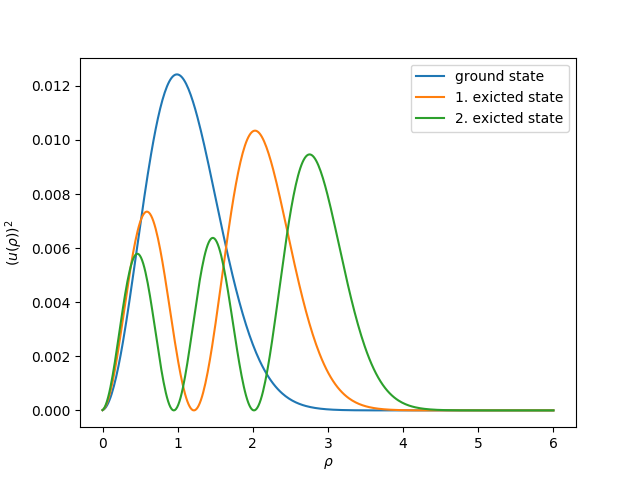
\includegraphics[width =1.2\textwidth]{solutions_one_electron_1_000000.png}
	\caption[Eigenfunctions$^2$ for one electron]{Square of the first three normalized eigenfunctions for one electron in the three-dimensional harmonic oscillator well as function of distance}
\end{figure}
From figure 1, one can also see the quantum mechanical occurrence of nodes. The first excited state has one node (that is, the squared wave function is zero), the second excited state has two, and so on. This is expected and follows quantum mechanical rules [4].
 
\subsection{two electrons in three-dimensional harmonic oscillator well}
As discussed before, the equation that needs to be solved is almost the same as for one electron, but with an extra term that leads to interesting observations. In order to see what happens, we compared the eigenvalue of the ground state with the Coloumb potential either turned on or turned off (which is the same as ignoring electron-electron repulsion. The electron-electron distance is then mathematically equal to the distance of one electron to the origin). We did this for several values of the  $\omega$, as can be seen in table 2:
\begin{table}[H]
\caption[Ground state eigenvalues for one and two electrons]{Ground state eigenvalue (unitless) for different values of $\omega$ for one electron ($\lambda_1$) or two electrons ($\lambda_2$)}
\begin{tabular}{lll}
$\omega$ &$\lambda_1$ & $\lambda_2$  \\
0.010 & 0.030 & 0.106 \\
0.500 &1.500 & 2.230 \\
1.000 &3.000 & 4.058  \\
5.000 &14.999 & 17.448\\
\end{tabular}
\end{table}
The relative difference between the eigenvalues get smaller for higher values of $\omega$ (which is related to the strength of the harmonic potential). This is probably caused by the Coloumb repulsion dominating for very small values of $\omega$, while the harmonic potential dominates for large values of $\omega$. \\
As can be seen in the appendix, the maximum value of the squared ground state wave function is stretched out to larger values of $\rho$ when the potential well is turned on. The position of the function's maximum with and without the Coloumb potential can be seen in table 3 (appendix), which gives similar results as the comparison of eigenvalues - a stronger potential leads to less difference between the eigenvalues. Figure 3 in the appendix illustrates that. It is worth mentioning again that the values for $\omega=0.01$ are not completely correct due to the wave function not flattening out even for $\rho$=40, as can be seen in the appendix.
\begin{figure}[H]
	\includegraphics[width =1.2\textwidth]{ground_state_comparision_omega_1_000000.png}
	\caption[Ground states of the single- and double- electron systems]{Ground states of the single- and double- electron systems compared under $\omega =1.000$}
\end{figure}

\section{Conclusion}

\section{Critique}

\section{Appendix}
\subsection{Proof that orthogonal transformations persever orthogonality of eigenvectors}\label{eigenvector orthogonality}
Let $v_i, v_j$ be the eigenvectors of a symmetric matrix A. They are orthogonal because A is symmetric, that is, $v_{j}^Tv_i$=0. Let U be an orthogonal matrix. The orthogonal transformation of the vector $v$ will retain its orthogonality because
 $(Uv_j)^T(Uv_i)=v_{j}^TU^TUv_i=v_{j}^T(U^TU)v_i=v_{j}^Tv_i=0$
\subsection{Proof that similar matrices share eigenvalues}\label{proof of same eigenvalues}
If a matrix $B$ is similar to a matrix $A$, then $B=S^{-1}AS$. Then if $\vec{x}$ is an eigenvector of $A$ with eigenvalue $\lambda$:
$$
A\vec{x}=\lambda\vec{x}
$$
Both sides of the equation can be multiplied by $S^{-1}$ and the identity operator $I = SS^{-1}$ can be inserted in between $A$ and $\vec{x}$ to yield
$$
S^{-1}ASS^{-1}\vec{x} =B\left(S^{-1}\vec{x}\right)= \lambda \left( S^{-1}\vec{x}\right)
$$
So $\lambda$ is also an eigenvalue of $B$ though with the corresponding eigenvector $\left( S^{-1}\vec{x}\right)$.
\subsection{Nondimensionalization of the radial Schroedinger equation for two interacting electrons}
\label{nondim_2_el}
Using the dimensionless variable $\rho=\frac{r}{\alpha}$ the equation becomes
\begin{equation*}
  -\frac{d^2}{d\rho^2} \psi(\rho) 
       + \frac{1}{4}\frac{mk}{\hbar^2} \alpha^4\rho^2\psi(\rho)+\frac{m\alpha \beta e^2}{\rho\hbar^2}\psi(\rho)  = 
\frac{m\alpha^2}{\hbar^2}E_r \psi(\rho) .
\end{equation*}
Introducing a new term 
$$
\omega_r^2=\frac{1}{4}\frac{mk}{\hbar^2} \alpha^4
$$
and defining $\alpha$ such that the term in front of 
$$
\frac{\psi(\rho)}{\rho}
$$
is $1$:
\begin{equation*}
\alpha = \frac{\hbar^2}{m\beta e^2}.
\end{equation*}
Defining the final eigenvalue
\begin{equation*}
\lambda = \frac{m\alpha^2}{\hbar^2}E_r,
\end{equation*}

\subsection{List of programs}
All programs can be found on \url{https://github.com/adrian2208/FYS3150_collab} in the map "project 2".
\begin{itemize}
\item[1.] catch.hpp - Neccessary library for unit testing
\item[2.] solve\_harmonic\_oscillator.cpp - takes n as input. Solves the buckling beam eigenvalue problem.
\item[3.] solve\_harmonic\_oscillator\_armadillo.cpp - takes n as input. Solves the buckling beam eigenvalue problem with armadillo.
\item[4.] solve\_one\_electron.cpp - takes n, rhomax and omega as input. Solves the eigenvalue problem for the harmonic oscillator potential with one electron.
\item[5.] solve\_two\_electrons.cpp -  takes n, rhomax and omega as input. Solves the eigenvalue problem for the harmonic oscillator potential with two electrons.
\item[6.] vecop.hpp and vecop.cpp - functions and algorithms.
\item[7.] tests.cpp - Unit testing.
\item[8.] tests\_main.cpp - Unit testing.
\item[9.] compile\_and\_run.py - Compiles and runs several .cpp files for several values of n and omega.
\item[10.] maxpeak.py - finds the $\rho$ value of the maximum of the wave function.
\item[11.] plot\_eigenvalue.py - The name says it. Also writes it to file.
\item[12.] plot\_solutions.py - Plots the eigenfunctions for a .txt file (which ones: To be specified in program).
\item[13.] plot\_two\_in\_one - Opens several files and plots the wave functions.
\end{itemize}

\subsection {Plots of eigenfunctions}
\begin{figure}[H]
	\includegraphics[width =1.2\textwidth]{solutions_two_electrons_0_010000.png}
	\caption[Approximated first 3 states for two electrons for $\omega$=0.01]{The first 3 states of the wave function for two electrons for $\omega$=0.01. One can clearly see how the wave functions are unnaturally shortened, and how even the ground state is not sufficiently zero.}
\end{figure}
\subsection{Tables}
\begin{table}[H]
\caption[Maximum value of eigenfunctions$^2$]{Position of maximum value of squared eigenfunctions expressed in $\rho$ (unitless) as a function for different values of $\omega$ for one electron ($\lambda_1$) or two electrons ($\rho_2$). It is worth noticing that the maximum value can be interpreted as the most likely distance between the two electrons / the electron and origo.}
\begin{tabular}{lll}
$\omega$ &$\rho_1$ & $\rho_2$  \\
0.010 & 9.962 & 18.273 \\
0.500 &1.411 & 1.667 \\
1.000 &0.992 & 1.128  \\
5.000 &0.441 & 0.471\\
\end{tabular}
\end{table}

\section{References}
\begin{itemize}
\item[(1)] Jacobi, C.G.J. (1846). "Über ein leichtes Verfahren, die in der Theorie der Säkularstörungen vorkommenden Gleichungen numerisch aufzulösen". Crelle's Journal (German)
\item[(2)] Morten Hjort-Jensen \textit{Computational Physics: Lecture Notes Fall 2015}
\item[(3)]G. Golub, C. Van Loan, Matrix Computations (John Hopkins University Press, 1996)
\item[(4)]David J. Griffiths, Darrell F. Schroeter, Introduction to Quantum Mechanics, third edition (Cambride University Press, 2018)
\item[(5)] FYS3150/FYS4150 Project 2 problem sheet "http://compphysics.github.io/ComputationalPhysics/doc/Projects/2019/Project2/pdf/Project2.pdf"
\end{itemize}


\begin{comment}

$$
\begin{bmatrix}
0 & 0 & 0 & 0 \\
0 & 0 & 0 & 0 \\
0 & 0 & 0 & 0 \\
0 & 0 & 0 & 0 \\
\end{bmatrix}
$$

\begin{lstlisting}[caption=insert caption]
for (unsigned int i = 0; i<100;i++{
}
\end{lstlisting}

\begin{figure}[h]
\includegraphics[width=8cm]{}
\caption{include caption}
\end{figure}

\end{comment}

\end{document}